\chapter{Cycles (30 pages)}
\label{Cycles}

\epigraph{"I don't know what you mean by 'glory,'?" Alice said.

Humpty Dumpty smiled contemptuously. "Of course you don't -- till I tell you. I meant 'there's a nice knock-down argument for you!'?"

"But 'glory' doesn't mean 'a nice knock-down argument'," Alice objected.

"When I use a word," Humpty Dumpty said, in rather a scornful tone, "it means just what I choose it to mean -- neither more nor less."

"The question is," said Alice, "whether you can make words mean so many different things."

"The question is," said Humpty Dumpty, "which is to be master, that's all."

--Lewis Carroll\\

I can't say `It's cold here' and mean `It's warm here' -- at least, not without a little help from my friends.\\--David Lewis}


We are now in a position to bring the formal framework developed in Section \ref{Signaling} to bear on the use of emphatic negation and its role in Jespersen's Cycle. We begin by first mapping the components discussed in Section \ref{Background} onto the structure of a signaling game. The possibility of different preferences for speakers and hearers is incorporated into the structure of the model. We determine the existence of evolutionarily stable strategies and note the transfer of information as the interests of speaker and hearer diverge. As the preferences of speakers and hearers diverge signaling becomes less informative. For sufficiently low differences, signaling remains informative, but beyond a certain point signaling collapses into uninformative pooling. We then consider the impact of introducing new signals, which lead to a kind of push-chain where the least informative signal is lost. Throughout, we discuss the implications of the model for Jespersen's Cycle.

\section{Emphasis}

\subsection{Signaling Game}

To begin, we must first consider how signaling games capture the use of negation. As we noted above, the difference between plain and emphatic negation is captured by the standard of precision applied. The speaker has knowledge about some state of the world which renders a particular negative expression acceptable on some standards, but not necessarily on others. Thus, there exists a continuum of states for the speaker, which we will take to be the interval $T = [0,1]$. The lowest possible value on such an interval corresponds to the weakest possible standard of precision that would still render the negative expression acceptable.\footnote{Here we leave out the possibility of the use of a given expression in the absence of any standard of precision being met. That is, we leave out cases of outright lying. Such cases are particularly interesting, but we leave them as a consideration for future study.} The highest possible value on the interval is then the strictest possible standard of 
interpretation available. 

Given that the speaker has observed some state of affairs, $t \in T$, he must choose a message, $m \in M$, to send to the hearer. Let $\mathcal{P}_n(T)= 0 < ... < t_{n-1} < ... < 1$ be a partition of the state space into $n$ subintervals.  A speaker's strategy is then a function from a partition of the type space to messages, $S : [\mathcal{P}_n(T) \rightarrow M]$. Intuitively, this is simply a way of carving up the state space into discrete regions and using those regions to determine which signal to send. For example, the trivial partition, $\mathcal{P}_1(T)$, occurs when the sender pools all types together and uses only a single message. In what follows we will largely be concerned with partitions of at least size two $\mathcal{P}_2(T)$. For example, consider the case of two messages, consisting of just a plain and an emphatic form. Letting $\mathcal{P}_2(T) = 0 < t_1 < 1$, a possible sender strategy is then  $s(t) = m_1$ for $t \in (0,t_1)$, and $s(t) = m_2$ for $t \in (t_1,1)$. That is, the sender uses 
$m_1$ for all types in the first subinterval, and $m_2$ for the second subinterval. Intuitively, we would refer to $m_1$ as the plain form of negation and $m_2$ as the emphatic.

Once the speaker has sent a message, the hearer is faced with the problem of how to interpret it. Given that the hearer cannot read the speaker's mind, she must infer the state of affairs that prompted the use of a particular form. That is, given the information conveyed by the signal, she must do her best to determine the standard of precision that warrants the speakers assertion. We will take the space of possible interpretations available to the hearer to be equivalent to the type space of the speaker, $A = [0,1]$. This representation captures the fact that the interpretation of expressions is not an all or nothing affair, but rather a matter of degrees.  A hearer's strategy is then a mapping from messages to interpretations, as above, $R : [M \rightarrow A]$.


\begin{figure}
\begin{center}
\begin{tikzpicture}[->,>=stealth',shorten >=1pt,auto,node distance=3cm]
  \node (A)      {$t_0$};
  \node (B) [right of=A]  {$m_0$};
  \node (C) [right of=B] {$a_0$};
  \node (D) [below of=A] {$t_1$};
  \node (E) [right of=D] {$m_1$};
  \node (F) [right of=E] {$a_1$};
\path[->] (A) edge node {$s_0^0$} (B)
	  (A) edge[dashed,pos=0.85] node {$s_0^1$} (E)
	  (B) edge node {$r_0^0$} (C)
	  (B) edge[dashed,pos=0.85] node {$r_0^1$} (F)
	  (D) edge[below] node {$s_1^1$} (E)
	  (D) edge[dashed,pos=0.75] node {$s_1^0$} (B)
	  (E) edge[below] node {$r_1^1$} (F)
	  (E) edge[dashed,pos=0.75] node {$r_1^0$} (C);
\end{tikzpicture}
\end{center}
\caption{Probabilities of actions in signaling game}
\label{probs}
\end{figure}

\begin{figure}
\begin{center}
\begin{tikzpicture}[->,>=stealth',shorten >=1pt,auto,node distance=3cm]
  \node (A)      {$t_0$};
  \node (B) [right of=A]  {$m_0$};
  \node (C) [right of=B] {$a_0$};
  \node (D) [below of=A] {$t_1$};
  \node (E) [right of=D] {$m_1$};
  \node (F) [right of=E] {$a_1$};
%  \node (G) [below of=D] {$t_2$};
\path[->] (A) edge node {$s_0^0$} (B)
	  (A) edge[dashed,pos=0.85] node {$s_0^1$} (E)
	  (B) edge node {$r_0^0$} (C)
	  (B) edge[dashed,pos=0.85] node {$r_0^1$} (F)
	  (D) edge[below] node {$s_1^1$} (E)
	  (D) edge[dashed,pos=0.75] node {$s_1^0$} (B)
	  (E) edge[below] node {$r_1^1$} (F)
	  (E) edge[dashed,pos=0.75] node {$r_1^0$} (C);
\end{tikzpicture}
\end{center}
\caption{Probabilities of actions in signaling game}
%\label{probs}
\end{figure}



With the definition of the strategies available to speakers and hearers, we can ask what kinds of preferences both might have over the correspondence between actual and inferred standards. It is uncontroversial that hearers are in the business of doing their best to accurately infer the actual state of affairs that prompted the signal. That is, hearers prefer their interpretation to be as close as possible to the standard of precision that the speaker actually has evidence for.  If it were otherwise, the existence of language would be truly puzzling from an evolutionary perspective; the gullible are not long for the tooth and claw world. So, if hearers are interested in the accurate transmission of information, then any misalignment must come from speakers' preferences. 

From the perspective of the speaker, we can adduce at least two related reasons why speakers might prefer overestimation. The first imputes a kind of categorical bias on the part of speakers, whereas the second relaxes this bias towards reasonability. We address them each in turn. First, we consider what the goals of communication are. Arguably, our chief goal in uttering a given expression is to affect some response in our interlocutors. In the case of a declaration we might think of this in terms of how convinced the hearer is after hearing an utterance. Or, in the terms we have developed thus far, we want the hearer to infer a particular standard of precision. We could take this preference as categorical. Namely, that regardless of the actual standard of precision, speakers want hearers to infer the absolute highest standard of precision possible. Given such a preference and a choice between signals that hearers respond to differentially, speakers will always choose the form that elicits the higher 
standard.  Speakers are, so to speak, on the lookout for the form that gives them the most bang for their breath. It should be noted that this bias is stipulative only insofar as it arises from the fundamental way we use words to do things.

Second, while this bias may naturally exist, it need not be categorical. Rather, speakers may simply prefer that hearers infer a standard of precision that is at least is strict as their own. This can be taken as a natural corollary of the inferential nature of communication. Hearers cannot read minds, and thus they must make some inference about the actual standard of precision. Speakers have only an indirect influence on this process of inference. Thus, they may wish to hedge their bets in a particular direction. Namely, they may want the inferred standard to be at least as strict as there own because it ensures that their own beliefs stand in a particular relation to hearers'. That is, the hearer's beliefs probabilistically entail those of the speaker.

The impact of this relationship is particularly clear with regard to perlocutionary concerns. For example, imagine the case where the issuer of one of the following threats has absolutely no desire to follow through on it.

  \ex. \a. If you move, I'll shoot.
       \b. If you budge an inch, I'll shoot.

By using the stronger threat, leading the hearer to infer a stricter standard than actually holds, the speaker has a better chance of not being forced to follow through on it. That is, the hearer will restrict his actions to those that do not constitute movement at the stricter standard, thus guaranteeing that they will not at the weaker actual standard. 

The same concerns hold in far more magnanimous circumstances. For example, in the case of offering a friend genuine advice on dining options, one might deem a mediocre restaurant one of the following.

 \ex. \a. Not good.
      \b. Not worth a cent!

While clearly hyperbole, the latter, much like the strong threat, offers a means for speakers to guide a friend to a good meal. In both cases, when hearers underestimate the standard of precision, the speaker runs the risk of not achieving his goals with resulting dire or not so delicious consequences. In contrast, these goals are guaranteed when hearers overestimate the standard of precision.

We can encode this slight bias in the utility functions of senders and receivers. As a means of parameterizing this possibility, we define the sender and receiver utility functions as a pair of quadratic functions, as in \cite{crawford-sobel:1982}, where $b \in [0,1]$ reflects the bias of the sender.\footnote{This bias need not be constant. For example, we might suppose that the bias is uniformly distributed over the interval $(t,t+b)$. This would capture the intuition that some of the time a speaker prefers overestimation of the standard, but not others. All of the following result hold for this more general case. As a preview, the only change below is that partial pooling equilibrium is defined at $t^* = \frac{1}{2} - 3b$ }

\begin{equation}
\begin{split}
     U_S(t, a) &= -(a - t - b)^2\\
  	 U_R(t, a) &= -(a - t)^2
\end{split}
\end{equation}
These utility functions reflect two intuitions. First, for a given type of sender, there is an action that maximizes the receiver's payoff. That is, the receiver does best by taking the action that is closest to the sender's type. Second, for a sender with a particular type, the action that maximizes the sender's payoff is offset by some bias, $b$. That is, the sender prefers the receiver to take the action she thinks appropriate for some higher type. In this case, $b$ represents the degree to which the sender wishes to exaggerate his type, if the receiver believes such exaggerations. When $b=0$ the interests of senders and receivers are completely aligned, but as $b$ grows, they diverge. This parallels the intuition that hearers are trying to infer the standard of precision for a given assertion, and prefer this to be as accurate as possible. It also reflects the fact that speakers have a slight preference for hearers to overestimate the standard of precision.

The impact of the sender's bias can be visualized as in Figure \ref{receiver_payoff}. For a sender with information $t=0$, the receiver would do best to take the action that accurately picks out the sender's state. In contrast, the sender's most preferred action is offset by the amount of bias. In the case where $b=\frac{1}{2}$, then the sender prefers the speaker to take an action higher than the receiver would prefer. This mismatch is only exacerbated as the amount of bias increases, as can be seen for the case where $b=1$. Visually speaking, as the bias increases, the utility functions of the sender and the receiver move away from each other. 


\begin{figure}
\begin{center}
\begin{tikzpicture}
\node (left) at (-1, 2)    {\includegraphics[width=.15\textwidth]{left.jpg}};
%draw horizontal line
\draw (0,0) -- (6,0);
%draw ticks
\draw (0,3pt) -- (0,-3pt);
\draw (6,3pt) -- (6,-3pt);
%draw tick labels
\draw (0,0) node[below=3pt] {\textsc{discourse new} } ;
\draw (6,0) node[below=3pt] {\textsc{discourse old} } ;
%
\draw (3,3pt) -- (3,-3pt);
\node (state) at (3, 1)    {$t$};
%
\draw (5,3pt) -- (5,-3pt);
\node (state) at (5, 1)    {$t+b$};
\draw [ultra thick] (3,1.5) to (5,1.5);
\node (state) at (4, 1.75)    {$b$};
\end{tikzpicture}     
\end{center}
\caption{$p :$ The plumber came.}
\end{figure}

\subsection{Equilibria}

For a given pair of sender and receiver strategies we can calculate the expected utility. In what follows we will assume that types are uniformly distributed over the interval, which yields the following expected utilities. Note that these are exactly parallel to expected utilities in a discrete state space presented above.

\begin{equation}
\begin{split}
     E[U_S(s, r)] &= \int_T -(r(s(t)) - t - b)^2 dt\\
      E[U_R(s, r)] &= \int_T -(r(s(t)) - t)^2 dt
\end{split}
\end{equation}

Now, we want to determine the conditions for equilibria. By doing so, we are determining what kinds of behavior we would expect on the part of speakers and hearers given the speaker's bias. That is, we want know how speakers will use different forms to signal standards of precision and how hearers will interpret them. The existence of different equilibria and their relative stability are crucial to the dynamics of Jespersen's Cycle.

Consider the potential equilibrium strategy profile $\langle s^*, r^* \rangle$. Let $s^*$ induce a partition of type $\mathcal{P}_2(T)$, where $t^*$ is the relevant threshold that distinguishes the two messages. Let $s^*(t) = m_1$ for $t \in (0,t^*)$ and $s^*(t) = m_2$ for $t \in (t^*,1)$. Let $r^*(m_1) = a_1^*$ and $r^*(m_2) = a_2^*$. In words, the sender splits the type space in two and sends a unique message for each subinterval. These are the plain and the emphatic forms of negation, respectively. The receiver responds to these messages with a particular action.  These are the inferred standards of precision in response to the different forms.

The strategy profile is an equilibrium if the relevant strategies are joint best responses. We can determine this by simply taking the partial derivative of the relevant utility functions with regard to the relevant variables. For the receiver, this can be determined by considering what actions are the best response to the senders partition. This simply tells us how the receiver's inference depends on the sender's use of the different forms.

\begin{equation}
\frac{\partial}{\partial a_1^*}E[U_R(s, r)] = \frac{\partial}{\partial a_2^*}E[U_R(s, r)] = 0
\end{equation}
These values are uniquely satisfied when the following hold.

\begin{equation}
     \begin{split}
	  a_1^* &= \frac{t^*}{2}\\
	  a_2^* &= \frac{1 + t^*}{2}
     \end{split}
\end{equation}
Intuitively, this means that however the speaker splits up the standards of precision, the receiver should respond to the emphatic form by inferring a higher standard of precision and the plain form with a lower standard of precision. The exact placement of these responses is determined by how the sender uses the signals. Namely, the hearer should infer the average standard of precision used for each of the two forms.

For the sender, we can proceed in a similar fashion determining when the following holds.
\begin{equation}
 \frac{\partial}{\partial t^*}E[U_S(s, r)] = 0
\end{equation}
This equation is satisfied when one of the following holds.

\begin{equation}
     \begin{split}
 	t^* &= 0\\
	t^* &= \frac{3}{4}(a_1^* + a_2^*) - \frac{3}{2}b - \frac{1}{4}\\
	t^* &= 1
     \end{split}
\end{equation}

These constraints together give rise to three distinct systems of equation. Solving each for $t^*$, we find the following equilibrium solutions in terms of the bias of the sender.

\begin{equation}
\begin{split}
     t^* &= 0\\
     t^* &= \frac{1}{2} - 6b\\
     t^* &= 1
\end{split}
\end{equation}
Both the first and the last of these equilibria are pooling equilibria. That is, senders only ever use a single signal. In response to this, receivers take the action that maximizes their expected utility given the prior probability distribution over types. That is, they guess the expected value of the type space. They simply infer the average standard of precision.

In contrast, the middle equilibrium constitutes a partially separating equilibrium. It is only partially separating because the state space is infinite, while the message space is not. This means that every type cannot be fully revealed, but that some information is transferred. The amount of information transferred and the distinction between the partially separating and pooling equilibria can be characterized in information-theoretic terms \citep{shannon:1948}. In particular, we can think of the amount of information conveyed by a particular signal at equilibrium according to the \emph{Kullback-Leibler Divergence} \citeyearpar{kullback-leibler1951divergence}.

\begin{equation}
     D_{KL}(P || Q) = \int_{-\infty}^{\infty} log\left( \frac{p(x)}{q(x)}  \right)p(x) dx
\end{equation}
This serves as a measure for how much change is induced in the receiver by a particular message. That is, in our case $q(x)$ corresponds to the prior probability distribution over types, and $p(x)$ corresponds to the probability of a sender being of a particular type given the message. The more the message shifts the probability from the prior, the more information it conveys. And, the less a message shifts the probability from the prior, the less information it conveys. 

For example, taking either of the pooling equilibria as an example.  If senders use the same signal regardless of state, then the conditional probability is the same as the prior probability. This means that there is absolutely no change from the prior probability, and hence zero information is transmitted via the signal. In contrast, for any partially separating equilibrium, a particular message induces a shift from the prior probability, and thus conveys some information. We should note that the amount of information conveyed regarding the standard of precision is distinct from the propositional content of a given utterance. For example, in the case where speakers use only a single form of negation for all standards of precision, the hearer will have no information in addition to and exceeding the prior probability. However, she will know the propositional content of the utterance. In other words, she will know \emph{that} negation was used, but not \emph{how} it was used.


Information is transferred at equilibrium only if the partially separating equilibrium exists. This is the case when the sender's bias is sufficiently low. Namely, only if $b < \frac{1}{12}$. If the bias is too large, then the partially separating equilibrium collapses into the lower pooling equilibrium.  However, a partially separating equilibrium, if it exists, is the only evolutionarily stable strategy profile. To see this note that in any pooling equilibrium receivers can respond to an unused message with any action whatsoever without affecting their expected utility. This means that pooling equilibria are not strict Nash equilibria and are thus not stable to invasion or innovation. 

% For example, suppose that receivers responded to an unused message with an action $a > \frac{1}{2}$. All senders would then do better to use that previously unused message in a particular set of states, $(\frac{1}{2}(a + \frac{1}{2}), 1]$. In turn, receivers woul
% 
%  have an incentive to adjust their responses to the two messages. In turn, senders have an incentive to adjust to this adjustment, and so forth. This process of mutual adjustment ends at the evolutionarily stable partially separating equilibrium.

We have established an upper limit on the amount of bias that allows for two signals to be used informatively. If this bias is exceeded, then signaling collapses. A single message is used, but carries no information. In fact, for a given number of signals, $n$, there exists some level of bias, $b_n$, that allows for their informative use in a partially separating equilibrium based on a sender's partition of the type space, $\mathcal{P}_n$ \citep{crawford-sobel:1982}. As the number of signals increase, the amount of bias must decrease to allow for informativity, thus $b_2 > b_3 > ... > b_n$. Intuitively, as the preferences of senders and receivers approach each other a finer and finer partition of the space is possible.

\subsection{Dynamics}

So, what does this mean for Jespersen's cycle? Intuitively, the pragmatics of emphasis suggest that the population originally starts at a point where one form is used with a  very high standard of precision and another is used for all other standards. That is, emphatic negation is distinguished from plain negation in its contexts of use. We can determine what will happen to these two signals over time. Intuitively, under the game dynamics, the signals will converge to their equilibrium use.

Under the game dynamics, for any amount of bias, no matter how slight, the emphatic form will spread to lower and lower standards of precision until it reaches its equilibrium use. The amount of bias determines where this process stops. That is, if a partially separating equilibrium exists, then the emphatic form will expand to encompass all standards of the upper part of the partition. In other words, the emphatic will be \emph{attenuated}, but still carry some information.  If no separation is possible, the emphatic form will spread across all standards. In other words, the emphatic will be entirely \emph{bleached} of its emphasis. Note that in both cases the process can be characterized in information-theoretic terms. That is, as the emphatic form spreads to more and more standard it conveys less and less information. 

The stable coexistence of plain and emphatic negation for long periods of time suggest that the bias is sufficiently small to allow for at least two forms. This, however, raises the question of what destabilizes the system. The system must be disturbed by a push chain, whereby the signal used for the lowest subinterval is lost. More generally, imagine a system with bias $b_n$ at equilibrium. Now, suppose that a new signal is introduced, so that there are now $n+1$ signals. Clearly, the system is not stable. However, it will be carried back to some equilibrium by the game dynamics. The resultant equilibrium depends on the character of the signal that is introduced. Let $a'$ be the response of receivers to the new signal $m'$. All messages that receive a lower response than $a'$ will be pushed down, the lowest of these being pushed out of use completely.  In the case of Jespersen's Cycle, new signals enter with a high $a'$, and thus displace everything below. That is, they are emphatic and lead hearers to 
infer a high standard of precision. This means that all other forms lower in the scale will be pushed down and the lowest will be pushed out of existence, exactly like what we see in the actual instantiation of the cycle.

\subsection{Modeling}

\begin{figure}
\centering
     \includegraphics[width=\textwidth]{lump-plot1.pdf}
\caption{Proportion of \textit{\color{blue} ne...not} and \textit{\color{green} not}  versus  \textit{\color{red}  ne} over time}
\label{lump-plot1}
\end{figure}

\begin{figure}
\centering
     \includegraphics[width=\textwidth]{neg-year-lines.pdf}
\caption{Proportion of forms of negation in Negative Declaratives}
\label{neg-three-plot}
\end{figure}


\section{Information Structure}

The motivation of this project stems from particular hypotheses about the conditioning factors of negation in Jespersen's Cycle \citeyearpar{jespersen:1917}, which can be characterized by the transition from pre-verbal to embracing to post-verbal negation: \textsc{\color{red} neg V} $\rightarrow$ \textsc{\color{blue} neg V neg} $\rightarrow$ \textsc{\color{green} V neg}. In particular, \cite{hansen2009, hansen-visconti2009,hansen-visconti2012} have used historical corpora of French and Italian to show that the embracing form (\textsc{\color{blue} neg V neg}) is sensitive to the discourse status of the proposition being negated. Namely, the embracing form is restricted to instances where the proposition being negated is either \textsc{discourse old} or \textsc{inferrable}.

\cite{schwenter2005,schwenter2006} uses synchronic data from Brazilian Portuguese to demonstrate the sensitivity of negation to these distinctions. Consider the following scenario. Suppose that a husband and wife expect a plumber to come fix their leaky faucet while they are at work during the day. The husband arrives home before his wife to find a still leaky faucet. The wife arrives home shortly and the first thing her husband says is the following.

\exg.  O bombeiro \textsc{\color{red} n{\~a}o} \textsc{\color{red} Veio}.\\
         The plumber neg came\\
         ``The plumber didn't come."\\

\exg. \#O bombeiro \textsc{\color{blue}n{\~a}o} \textsc{\color{blue}Veio} \textsc{\color{blue}n{\~a}o}.\\
	The plumber neg came neg\\
	``The plumber didn't come."\\

The reason that the embracing form is odd is that it comes out of the blue, so to speak. That is, the proposition ``The plumber came.'' is entirely \textsc{discourse new}. Even if the husband has some expectation that his wife has been thinking about whether or not the plumber came, the proposition has not been introduced into the \emph{discourse} yet. The embracing form cannot be used to negate \textsc{discourse new} propositions.

However, how the proposition can be introduced into the discourse in several ways, both explicitly and implicitly. For example, if the wife walks in the door and says the following.

\exg.  O bombeiro veio hoje?\\
       The plumber came today\\
         ``Did the plumber come today?"\\

Asking the question has explicitly introduced the proposition into the discourse, making either form appropriate in the husband's response. In fact, the wife need not even explicitly ask the question. For example, if she arrives home and points quizzically at sink, then the embracing form is fine. This is because the proposition can be inferred from the discourse.

Schwenter shows that even finer distinctions can be made in the sensitivity of different forms of negation to discourse context. For example, consider the following scenario. Suppose that two colleagues meet in a departmental hallway in the afternoon after a scheduled talk, and one asks the other the following question.

\exg. Voc{\^e} gostou da palestra da Maria?\\
	 you liked the talk of Maria\\
	 ``Did you like Maria's talk?"

\exg. \textsc{\color{blue}N{\~a}o} \textsc{\color{blue}Fui} \textsc{\color{blue}n{\~a}o}.\\
	 neg went neg\\
	 ``I didn't go."\\

\exg. \#\textsc{\color{green}Fui} \textsc{\color{green}n{\~a}o}.\\
	  went neg\\
	 ``I didn't go."\\

The reason that the post-verbal form is odd is that the proposition being negated ``I went (to Maria's talk).'' is only indirectly connected to the discourse. That is, liking a talk presumably requires having attended it, so the proposition is only \textsc{inferrable} from the discourse. The post-verbal form cannot be used where the proposition is discourse new or inferrable. This is made clear by altering the form of the response to the question of liking the talk.

\exg. \textsc{\color{blue}N{\~a}o} \textsc{\color{blue}Gostei} \textsc{\color{blue}n{\~a}o}.\\
	 neg liked neg\\
	 ``I didn't like it."\\

\exg. \textsc{\color{green}Gostei} \textsc{\color{green}n{\~a}o}.\\
	  liked neg\\
	 ``I didn't like it."\\

In this case the post-verbal form is acceptable because the proposition ``I liked Maria's talk.'' has been introduced into the discourse by the original question. The conditions and restrictions on different forms can be summarized as in Table \ref{schwenter}. The pre-verbal form is acceptable in any context, but the other two forms are only acceptable in more and more restricted contexts,

\begin{table}
\begin{center}
\begin{tabular}{@{}ccccc@{}}
      \hline
       & \textsc{discourse new} & \textsc{inferrable} & \textsc{discourse old}\\ \hline
      \textsc{\color{red} neg V} & $\checkmark$ &  $\checkmark$ &  $\checkmark$ \\
      \textsc{\color{blue} neg V neg} & \#  & $\checkmark$ & $\checkmark$ \\
      \textsc{\color{green} V neg} & \#  & \#  & $\checkmark$ \\
      \hline
\end{tabular}     
\end{center}
\caption{Acceptability of forms in discourse contexts}     
\label{schwenter}
\end{table}


It is not entirely clear if the forms of negation in Brazilian Portuguese should be treated differently than the canonical cases of embracing negation in Jespersen's Cycle (cf. \emph{ne...pas} in French, \emph{ne...not} in English). However, languages with only the pre-verbal and embracing form have been shown to exhibit this same sensitivity to discourse status (e.g. \cite{schwenter2006} for Catalan and Italian, \cite{hansen2009} for French). Namely, languages that only have two forms make the distinction between \textsc{discourse new} and everything else. This, of course raises the question of whether the post-verbal form is necessarily sensitive to discourse status or is the result of other processes, such as phonetic reduction. These are open empirical questions, which might also vary by the particular circumstances of a language.

However, the general shape of the conditioning factors suggests an intuitive characterization Jespersen's Cycle. That is, the different forms of negation are sensitive to the scale of how closely the negated proposition is connected to the discourse. That is, if we take connection to the discourse as a continuous measure, then discourse new propositions are at the low end, discourse old propositions are at the high end, and inferrable propositions are somewhere in the middle. In fact, we can simply reduce this to a scale of degrees of inferrability: discourse new propositions are not inferrable since we can't read minds, and discourse old propositions are completely inferrable since they have just been explicitly introduced into the discourse. 

We can represent this visually as in Figure \ref{continuum}, where we have simply taken the discrete categories used to construct Table \ref{schwenter} and treated them as a continuum. In fact, this wording is potentially misleading. If discourse status is about beliefs, then the underlying phenomenon is essentially gradient in nature. The discrete categories are useful because they correspond to portions of the continuum. While we have robust intuitions about the discrete categories, the varying strength of these intuitions suggests that the underlying phenomenon is essentially gradient in nature.

\begin{figure}
     \begin{center}
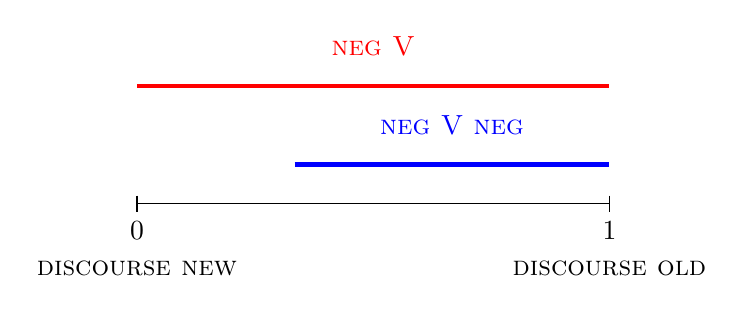
\begin{tikzpicture}
% \node (left) at (-1, 2)    {\includegraphics[width=.15\textwidth]{left.jpg}};
% \node (left) at (7, 2)    {\includegraphics[width=.15\textwidth]{right.jpg}};
%draw horizontal line
\draw (0,0) -- (6,0);
%draw ticks
\draw (0,3pt) -- (0,-3pt);
\draw (6,3pt) -- (6,-3pt);
%draw tick labels
\draw (0,0) node[below=3pt] {0} ;
\draw (6,0) node[below=3pt] {1} ;
\draw (0,-.5) node[below=3pt] {\textsc{discourse new} } ;
\draw (6,-.5) node[below=3pt] {\textsc{discourse old} } ;
%
\draw [ultra thick,red] (0,1.5) to (6,1.5);
\draw [ultra thick,blue] (2,.5) to (6,.5);
\draw (3,2) node {\textsc{\color{red} neg V}};
\draw (4,1) node {\textsc{\color{blue} neg V neg}};
% \draw (2,.25) node {$a_{\text{\textsc{\color{red} neg V}}}$};
% \draw (5,.25) node {$a_{\textsc{\color{blue} neg V neg}}$};

\end{tikzpicture}     
\end{center}
  \caption{Forms of negation given degree of inferrability}
  \label{continuum}
\end{figure}



The continuous representation also offers us some insight into \emph{why} Jespersen's Cycle occurs. The reasoning is as follows. First, keeping track of what is actually part of the discourse is difficult. In fact, this is the problem of \emph{common knowledge}\footnote{In epistemic logic \emph{mutual knowledge} only requires that everyone know that $p$, without any further steps. Thus anything that is common knowledge is also mutual knowledge, but not \emph{vice versa}. \cite{lewis:1969} introduced common knowledge in Philosophy. \cite{clark-marshall1981} use the term ``mutual knowledge'' to refer to common knowledge.}, that everyone knows that $p$, that everyone knows that everyone knows that $p$, \emph{ad infinitum}. \cite{clark-marshall1981} outline a set of reasonable heuristics for circumventing this infinite regress, including physical or linguistic co-presence and community membership. While these heuristics are made with reference to resolving the problem of common knowledge, they extend equally to 
propositions. Namely, propositions can be introduced to the discourse either explicitly (linguistic co-presence) or implicitly (physical co-presence, community membership).

Second, we have ample experimental evidence that speakers have particular biases in communication. Speakers tend to overestimate how successful they are at communication. \cite{savitsky-etal:2011} had two pairs of friends participate in a simple communication task. All four participants sat back to back and were individually given lists of four-way ambiguous sentences to read out loud with a specified meaning. For example, the sentence ``It's getting hot in here.'' could be interpreted as an indirect request to open the window or an amorous advance. Participants were asked to do two things. They were asked to guess the intended meaning of the sentences spoken by the other participants. They were also asked to estimate how many of the sentences the friend they came with had guessed correctly, and how many sentences the strangers from the other pair had guessed correctly. 

The results can be seen in Figure \ref{savitsky}. Listeners were reliably above chance at guessing the intended meaning out of the four potential meanings, but, friends and strangers did not differ significantly. However, speakers had much higher expectations  for listeners, significantly overestimating how many sentences listeners would accurately guess. This suggests that, as speakers, we often tend to overestimate how transparent our utterances actually are to our listeners.


\begin{figure}
\begin{center}
\includegraphics[width=.7\textwidth]{savitsky.pdf}          
\end{center}
  \caption{Results from \cite{savitsky-etal:2011}}
   \label{savitsky}
\end{figure}


\cite{lane-etal2006} offer evidence that is particular germane to the question of discourse status. The experimental design can be seen in Figure \ref{elephants-exp}. Participants were assigned the role of either the speaker or addressee in a communication game. Speakers were instructed to communicate information about a target shape to the addressee. One shape was visible to only the speaker, blocked from the view of the addressee by an occluder. In the target conditions, the item that was visible only to the speaker was the same shape, but varied along some relevant dimension (e.g. size, color). Figure \ref{elephants-results} shows the proportion of trials where speakers used a modifier in referring to the target item. Surprisingly, speakers' privileged information leaks into what is said. In fact, this happens to an even greater extent when speakers were explicitly instructed to conceal information about their privileged information.


\begin{figure}
\begin{center}
\includegraphics[width=.7\textwidth]{elephants-exp.png}          
\end{center}
  \caption{Experimental design of \cite{lane-etal2006}}
   \label{elephants-exp}
\end{figure}


\begin{figure}
\begin{center}
\includegraphics[width=.7\textwidth]{elephant-results.png}          
\end{center}
  \caption{Results for \cite{lane-etal2006}}
   \label{elephants-results}
\end{figure}

Returning to Jespersen's Cycle, we note that these experimental findings suggest a potential explanation for \emph{why} change takes place. The embracing form is restricted to a particular set of contexts where the proposition being negated is discourse old, or highly inferrable. If speakers tend to overestimate how inferrable the proposition being negated is, if they fail to filter out their own privileged information, then they will tend to use the embracing form in less and less inferrable contexts. The result will be an increase in the frequency of the embracing form over time. \cite{ahern-clark2015} offer a formal model of the dynamics of this process. However, the predictions of the model, like the corpus work by \cite{hansen2009, hansen-visconti2009}, are largely qualitative. That is, they demonstrate that the different forms of negation are sensitive to different constraints at different points in time, and offer an explanation of why those constraints might change over time. However, they offer no 
quantitative predictions about the shape of the change.

In contrast, \cite{wallage2013} presents a quantitative analysis of the conditioning factors of Jesepersen's Cycle in Middle English, drawing on evidence from the Penn Parsed Corpus of Middle English \citep{ppcme2}. Wallage codes sentences containing sentential negation for the discourse status of the proposition being negated, according to the categories outlined above. From two separate statistical tests on binned data (1150-1250 and 1250-1350), Wallage argues that if we factor out the overall rate of the embracing form, the effect of discourse status is not different across the two time bins. While the argument is interesting and it has great merit in being quantitative, the methodology is not compelling. That is, Wallage uses a form of \href{http://en.wikipedia.org/wiki/Variable_rules_analysis}{VARBRUL} and claims that the coefficients across discourse contexts are similar enough. There are several problems with this approach. First, it doesn't offer any way of quantitatively specifying how similar is 
similiar \emph{enough}. While regular practice may yield some insight, we want a statistical measure of how similar is similar enough to not reject the hypothesis that the conditioning of discourse status changes. Second, binning the data and not accounting for the potential effects of individual documents may yield misleading results. More appropriate methods, such as generalized linear mixed-effects models (GLMMs) would be more appropriate, and Wallage (p.c.) is moving towards the application of these new statistical techniques.

As it stands though, we don't have a clear answer to whether Jespersen's Cycle is driven by a sensitivity to discourse functional constraints. There are at least two potential explanations that reconcile the findings of \cite{hansen2009, hansen-visconti2009}, the experimental evidence of \cite{lane-etal2006}, the formal model of \cite{ahern-clark2015}, and the null result of \cite{wallage2013}. First, the role of discourse stats in Jespersen's Cycle may differ across languages. That is, the fact that the negation is sensitive to information structure may be particular to Romance languages. In fact, these constraints have only been noted in Romance languages. This could be the result of the constraints only occurring in Romance languages or just a lack of investigation into other languages synchronically and diachronically. The fact that the discourse status conditions in English don't change over time could be explained by this. However, it's striking that, at the beginning of the change, the embracing form 
in English is largely restricted to Inferrable and Discourse Old contexts. It would be surprising if this were a simple coincidence. Second, absent an explicit model of how and \emph{why} the discourse status constraints might be changing, the methodology employed by Wallage does not tell us much. That is, Wallage implicitly adopts the null hypothesis that the rate of change across discourse contexts is not different and argues that this null hypothesis cannot be rejected. However, it is not entirely clear what the null hypothesis ought to be, or if his method can actually tell us when we can reject it.

While we are still left with a fair amount of uncertainty regarding the actual causes of the cycle, it's clear that answering it will require a quantitative analysis of the conditioning factors of different forms of negation. The downside in this regard is that discourse status is not necessarily a surface property of sentences. That is, we cannot simply take a sentence and read off its relation to the previous discourse. Coding for discourse status requires a careful consideration of the prior context, the potential interpretations of a sentence, and general knowledge about the world.  This task is not straightforward even when analyzing contemporary language equipped with modern intuitions. The difficulty is only exacerbated when we turn to historical corpora. This leads to a reliance on expertise in the historical forms of a language to even perform a qualitative analysis, and a substantial investment of time and expertise to hand-code a large enough set of data to perform a quantitative statistical 
analysis. Unfortunately, this means that a comprehensive answer to the question of whether discourse constraints are important in Jespersen's Cycle is dependent on having experts in the history of multiple languages where the cycle has occurred invest a significant amount of time towards coding and evaluating the results. This is certainly possible, but also certainly a difficult task.

The goal of this project will be to explore methods for circumventing the need for significant expertise in the history of a language and significant time to understand the role of discourse status in change. In particular, we will be searching for surface properties of sentences that correlated with discourse status. On the assumption that these other surface properties stand in a stable relation to discourse status, we can probabilistically predict the discourse status of particular forms over time. That is, we are trying to infer the surface proxies of discourse status so that we can at least partially automate the process of determining the role of discourse in change. In the next section we describe the methods and data we will use.

\subsection{Signaling Game}

\subsection{Equilibria}

\subsection{Dynamics}

\subsection{Modeling}


%\section{Future Directions}
%
%This analysis suggests how Jespersen's Cycle can arise from signaling under a slight speaker bias. Examining the effect of these pragmatic pressures we established the following results. First, we showed that, for any amount of bias, emphatic forms become less informative over time. The extent of this loss is governed by the amount of bias, ranging from attenuation to complete bleaching. Second, only finitely many signals are stable in equilibrium for a given amount of bias.  The introduction of additional signals results in a push-chain scenario whereby the least informative signal is lost and the population returns to equilibrium. 
%
%There are several further directions that remain to be explored. First, we have encoded a bias on the part of the speaker into the utility function. This gives rise to the inflationary effect whereby emphatic negation is attenuated. However, it is not clear that this effect need arise from the speaker's preferences. For example, it may be the case that it could equally as well arise from the speaker's uncertainty regarding the hearers beliefs about the distribution over standards of precision. Thus far, we have relied on the \emph{common prior assumption}, which allows for the reduction of games of incomplete information to games of imperfect information \citep{harsanyi:1967,harsanyi:1968a,harsanyi:1968b}. That is, we have assumed that both speaker and hearer share the same prior probability over standards of precision. This need not be the case, but it is an open question as to whether removing this restriction yields a qualitatively different result than the course pursued here. Further, given every 
%individual's experience as both a sender and a hearer, the common prior assumption may be well justified.
%
%Second, we have assumed a uniform prior distribution over the state space. This serves well enough as a starting point, but the interaction between distributions and biases may yield dramatically different constraints than those discussed above. A straightforward generalization could be had by considering the \emph{Beta Distribution} over the state space, of which the uniform distribution is a special case. This would allow for a wide ranging test of the interaction between the prior probability and the amount of information that can be conveyed. Finally, the generalization of the prior can be informed in part by an empirical investigation of how often emphatic negation actually occurs. For example, if, as we have suggested, emphatic negation arises from NPIs in focus then we should be able to estimate the overall rate of use by determining how often such NPIs bear the mark of an abstract focus feature. That is, we can compare the overall rate of negation to the occurrence of NPIs with prosodic prominence.  
%While this only indirectly tells us about the underlying distribution of standards of precision, it provides a kind of constraint that will allow us to estimate likely distributions.
